%package list
\documentclass{article}
\usepackage[top=3cm, bottom=3cm, outer=3cm, inner=3cm]{geometry}
\usepackage{multicol}
\usepackage{graphicx}
\usepackage{url}
%\usepackage{cite}
\usepackage{hyperref}
\usepackage{array}
%\usepackage{multicol}
\newcolumntype{x}[1]{>{\centering\arraybackslash\hspace{0pt}}p{#1}}
\usepackage{natbib}
\usepackage{pdfpages}
\usepackage{multirow}
\usepackage[normalem]{ulem}
\useunder{\uline}{\ul}{}
\usepackage{svg}
\usepackage{xcolor}
\usepackage{listings}
\lstdefinestyle{ascii-tree}{
    literate={├}{|}1 {─}{--}1 {└}{+}1 
  }
\lstset{basicstyle=\ttfamily,
  showstringspaces=false,
  commentstyle=\color{red},
  keywordstyle=\color{blue}
}
%\usepackage{booktabs}
\usepackage{caption}
\usepackage{subcaption}
\usepackage{float}
\usepackage{array}

\newcolumntype{M}[1]{>{\centering\arraybackslash}m{#1}}
\newcolumntype{N}{@{}m{0pt}@{}}


%%%%%%%%%%%%%%%%%%%%%%%%%%%%%%%%%%%%%%%%%%%%%%%%%%%%%%%%%%%%%%%%%%%%%%%%%%%%
%%%%%%%%%%%%%%%%%%%%%%%%%%%%%%%%%%%%%%%%%%%%%%%%%%%%%%%%%%%%%%%%%%%%%%%%%%%%
\newcommand{\itemEmail}{wroquequi@unsa.edu.pe}
\newcommand{\itemStudent}{William Isaias Roque Quispe}
\newcommand{\itemCourse}{Programación Web 2}
\newcommand{\itemSemester}{III}
\newcommand{\itemUniversity}{Universidad Nacional de San Agustín de Arequipa}
\newcommand{\itemFaculty}{Facultad de Ingeniería de Producción y Servicios}
\newcommand{\itemDepartment}{Departamento Académico de Ingeniería de Sistemas e Informática}
\newcommand{\itemSchool}{Escuela Profesional de Ingeniería de Sistemas}
\newcommand{\itemAcademic}{2023 - A}
\newcommand{\itemInput}{Del 8 junio 2023}
\newcommand{\itemOutput}{Al 14 Junio 2023}
\newcommand{\itemPracticeNumber}{05}
\newcommand{\itemTheme}{Django}
%%%%%%%%%%%%%%%%%%%%%%%%%%%%%%%%%%%%%%%%%%%%%%%%%%%%%%%%%%%%%%%%%%%%%%%%%%%%
%%%%%%%%%%%%%%%%%%%%%%%%%%%%%%%%%%%%%%%%%%%%%%%%%%%%%%%%%%%%%%%%%%%%%%%%%%%%

\usepackage[english,spanish]{babel}
\usepackage[utf8]{inputenc}
\AtBeginDocument{\selectlanguage{spanish}}
\renewcommand{\figurename}{Figura}
\renewcommand{\refname}{Referencias}
\renewcommand{\tablename}{Tabla} %esto no funciona cuando se usa babel
\AtBeginDocument{%
	\renewcommand\tablename{Tabla}
}

\usepackage{fancyhdr}
\pagestyle{fancy}
\fancyhf{}
\setlength{\headheight}{30pt}
\renewcommand{\headrulewidth}{1pt}
\renewcommand{\footrulewidth}{1pt}
\fancyhead[L]{\raisebox{-0.2\height}{
\includegraphics[width=3cm]{img/logo_episunsa.png}}}
\fancyhead[C]{\fontsize{7}{7}\selectfont	\itemUniversity \\ \itemFaculty \\ \itemDepartment \\ \itemSchool \\ \textbf{\itemCourse}}
\fancyhead[R]{\raisebox{-0.2\height}{
\includegraphics[width=1.2cm]{img/logo_abet}}}
\fancyfoot[L]{Estudiante: William Roque Quispe}
\fancyfoot[C]{\itemCourse}
\fancyfoot[R]{Página \thepage}

% para el codigo fuente
\usepackage{listings}
\usepackage{color, colortbl}
\definecolor{dkgreen}{rgb}{0,0.6,0}
\definecolor{gray}{rgb}{0.5,0.5,0.5}
\definecolor{mauve}{rgb}{0.58,0,0.82}
\definecolor{codebackground}{rgb}{0.95, 0.95, 0.92}
\definecolor{tablebackground}{rgb}{0.8, 0, 0}

\lstset{frame=tb,
	language=bash,
	aboveskip=3mm,
	belowskip=3mm,
	showstringspaces=false,
	columns=flexible,
	basicstyle={\small\ttfamily},
	numbers=none,
	numberstyle=\tiny\color{gray},
	keywordstyle=\color{blue},
	commentstyle=\color{dkgreen},
	stringstyle=\color{mauve},
	breaklines=true,
	breakatwhitespace=true,
	tabsize=3,
	backgroundcolor= \color{codebackground},
}

\begin{document}
	
	\vspace*{10px}
	
	\begin{center}	
		\fontsize{17}{17} \textbf{ Informe de Laboratorio \itemPracticeNumber}
	\end{center}
	\centerline{\textbf{\Large Tema: \itemTheme}}
	%\vspace*{0.5cm}	

	\begin{flushright}
		\begin{tabular}{|M{2.5cm}|N|}
			\hline 
			\rowcolor{tablebackground}
			\color{white} \textbf{Nota}  \\
			\hline 
			     \\[30pt]
			\hline 			
		\end{tabular}
	\end{flushright}	

	\begin{table}[H]
		\begin{tabular}{|x{4.7cm}|x{4.8cm}|x{4.8cm}|}
			\hline 
			\rowcolor{tablebackground}
			\color{white} \textbf{Estudiante} & \color{white}\textbf{Escuela}  & \color{white}\textbf{Asignatura}   \\
			\hline 
			{\itemStudent \par \itemEmail} & \itemSchool & {\itemCourse \par Semestre: \itemSemester}     \\
			\hline 			
		\end{tabular}
	\end{table}		
	
	\begin{table}[H]
		\begin{tabular}{|x{4.7cm}|x{4.8cm}|x{4.8cm}|}
			\hline 
			\rowcolor{tablebackground}
			\color{white}\textbf{Laboratorio} & \color{white}\textbf{Tema}  & \color{white}\textbf{Duración}   \\
			\hline 
			\itemPracticeNumber & \itemTheme & 04 horas   \\
			\hline 
		\end{tabular}
	\end{table}
	
	\begin{table}[H]
		\begin{tabular}{|x{4.7cm}|x{4.8cm}|x{4.8cm}|}
			\hline 
			\rowcolor{tablebackground}
			\color{white}\textbf{Semestre académico} & \color{white}\textbf{Fecha de inicio}  & \color{white}\textbf{Fecha de entrega}   \\
			\hline 
			\itemAcademic & \itemInput &  \itemOutput  \\
			\hline 
		\end{tabular}
	\end{table}
	
	\section{Tarea}
	\begin{itemize}
         \item Crea un blog sencillo en un entorno virtual utilizando la guía: \url{https://tutorial.djangogirls.org/es/django_start_project/}
         \item Especificar paso a paso la creación del blog en su informe.
         \item Crear un video tutorial donde realice las operaciones CRUD (URL public reproducible online)
         \item Adjuntar URL del video en el informe.
         \end{itemize}
		
	\section{Equipos, materiales y temas utilizados}
	\begin{itemize}
		\item Sistema Operativo 
		\item GNU Vim.
		\item Python 3.11.3.
		\item Git
		\item Cuenta en GitHub con el correo institucional.
		\item Entorno virtual.
            \item Django 4.
	\end{itemize}
	
	\section{URL de Repositorio Github}
	\begin{itemize}
		\item URL del Repositorio GitHub para clonar o recuperar.
		\item \url{https://github.com/WilliamIsaiasRoque/Lab05-Pweb2.git}
		\item URL para el laboratorio 05 en el Repositorio GitHub.
		\item \url{https://github.com/rescobedoq/pw2/tree/main/labs/lab05}
            \item URL del video subido en Flip.
            \item \url{https://flip.com/groups/14644257/topics/36914916/responses/429073515/comments}
	\end{itemize}
	
	\section{Actividades}

	\subsection{Crear un directorio para el entorno virtual}
	\begin{itemize}	
		\item En este directorio inicializaremos el git y agregaremos un primer commit para probar.
	\end{itemize}	
		
	\begin{lstlisting}[language=bash,caption={Creando directorio de trabajo y accediendo en él}][H]
		$ mkdir PWEB2lab/Lab05-Pweb2/
	\end{lstlisting}
	\begin{lstlisting}[language=bash,caption={Dirijiéndonos al directorio de trabajo}][H]
		$ cd PWEB2lab/Lab05-Pweb2/
	\end{lstlisting}	
	\begin{lstlisting}[language=bash,caption={Inicializando el repositorio Git y agregando remote add origin}][H]
		$ git init
		$ git remote add origin https://github.com/WilliamIsaiasRoque/Lab05-Pweb2.git
	\end{lstlisting}
        \begin{lstlisting}[language=bash,caption={Añadiendo un README.md como primer push}][H]
		$ echo "# Lab05-Pweb2" >> README.md
		$ git add README.md
		$ git commit -m "Initial commit"
		$ git push -u origin main
	\end{lstlisting}

        \subsection{Crear un entorno virtual en el directorio}
        \begin{lstlisting}[language=bash,caption={Creando el directorio django\_env y accediendo en esa carpeta}][H]
		$ mkdir django_env
		$ cd django_env
		$ virtualenv -p python env
	\end{lstlisting}        	
        \begin{lstlisting}[language=bash,caption={Activando el entorno virtual con source}][H]
		$ source env/Scripts/activate
	\end{lstlisting} 
        \begin{lstlisting}[language=bash,caption={Instalando Django con pip}][H]
		$ pip install Django
		$ pip list
		Package    Version
		---------- -------
		asgiref    3.7.2
		Django     4.2.2
		pip        23.1.2
		sqlparse   0.4.4
	\end{lstlisting}
        \begin{lstlisting}[language=bash,caption={Creando un proyecto Django llamado mysite}][H]
		$ django-admin startproject mysite
	\end{lstlisting} 
        
	\subsection{Commits}
	\begin{lstlisting}[language=bash,caption={Primero se crea una aplicación llamada blog}][H]
		$ python manage.py startapp blog
	\end{lstlisting}
	
	\begin{itemize}	
		\item Los commits más importantes aparecerán en esta sección, al final se mostrarán unas capturas con todos los commits.
	\end{itemize}
        \begin{itemize}	
		\item Se ha modificado myenv/settings.py porque se agregó 'blog.apps.BlogConfig' para la correcta creación de la aplicación. También se cambió la zona horaria a 'America/Lima'
	\end{itemize}
        \lstinputlisting[language=python, caption={src/mysite/settings.py},numbers=left,]{src/mysite/settings.py}
        \begin{itemize}	
		\item Se ha generado 'manage.py' cuando se creó el proyecto.
	\end{itemize}
        \lstinputlisting[language=python, caption={src/manage.py},numbers=left,]{src/manage.py}
        \begin{itemize}	
		\item Se ha creado el modelo de Post en blog/apps.py y se ha importado a blog/admin.py
	\end{itemize}
        \lstinputlisting[language=python, caption={blog/apps.py},numbers=left,]{src/blog/apps.py}
        \lstinputlisting[language=python, caption={blog/admin.py},numbers=left,]{src/blog/admin.py}
        \lstinputlisting[language=python, caption={blog/models.py},numbers=left,]{src/blog/models.py}
        \begin{itemize}	
		\item En el siguiente commit se aplicó makemigrations y migrate en el terminal, el código se generó automáticamente
	\end{itemize}
        \begin{itemize}	
		\item En mysite/urls.py se agregó 'include' a 'from django.urls import path'.
	\end{itemize}
        \lstinputlisting[language=python, caption={src/mysite/urls.py},numbers=left,]{src/mysite/urls.py}
        \begin{itemize}	
		\item Se he creado un html en blog/templates/blog/base.html y una hoja de estilo básica en blog/static/css/blog.css
	\end{itemize}
        \lstinputlisting[language=html, caption={src/blog/templates/blog/base.html},numbers=left,]{src/blog/templates/blog/base.html}
        \lstinputlisting[language=html, caption={src/blog/static/css/blog.css},numbers=left,]{src/blog/static/css/blog.css}
        \begin{itemize}	
		\item En el directorio raíz se agregó 'requirements.txt' para especificar las versiones utilizadas.
	\end{itemize}
        \lstinputlisting[language=bash, caption={src/requirements.txt},numbers=left,]{src/requirements.txt}
        \begin{itemize}	
		\item Creación de un form inicial que permite crear nuevos posts.
	\end{itemize}
        \lstinputlisting[language=python, caption={src/blog/forms.py},numbers=left,]{src/blog/forms.py}
        \begin{itemize}	
		\item Se ha agreado post\_list.html para la visualización de posts.
	\end{itemize}
        \lstinputlisting[language=html, caption={src/blog/templates/blog/post\_list.html},numbers=left,]{src/blog/templates/blog/post\_list.html}

        \begin{itemize}	
		\item Creación de nuevos html para las operaciones CRUD.
	\end{itemize}
        \lstinputlisting[language=html, caption={src/blog/templates/blog/post\_edit.html},numbers=left,]{src/blog/templates/blog/post\_edit.html}
        \lstinputlisting[language=html, caption={src/blog/templates/blog/post\_detail.html},numbers=left,]{src/blog/templates/blog/post\_detail.html}
        \lstinputlisting[language=html, caption={src/blog/templates/blog/post\_delete.html},numbers=left,]{src/blog/templates/blog/post\_delete.html}

        \begin{itemize}	
		\item Modificaciones en urls.py y views.py para los html creados anteriormente.
	\end{itemize}
        \lstinputlisting[language=python, caption={src/blog/urls.py},numbers=left,]{src/blog/urls.py}
        \lstinputlisting[language=python, caption={src/blog/views.py},numbers=left,]{src/blog/views.py}
        \begin{itemize}	
		\item Cabe aclarar que no se han agregado la mayoría de archivos de mysite, ya que no han sufrido ningún cambio en el archivo, tal es el caso de \_init\_.py , asgi.py y wsgi.py
        \end{itemize}
        \begin{itemize}	
		\item A continuación las capturas de todos los commits realizados en el repositorio GitHub
        \end{itemize}
        \begin{figure}[ht]
        \centering
        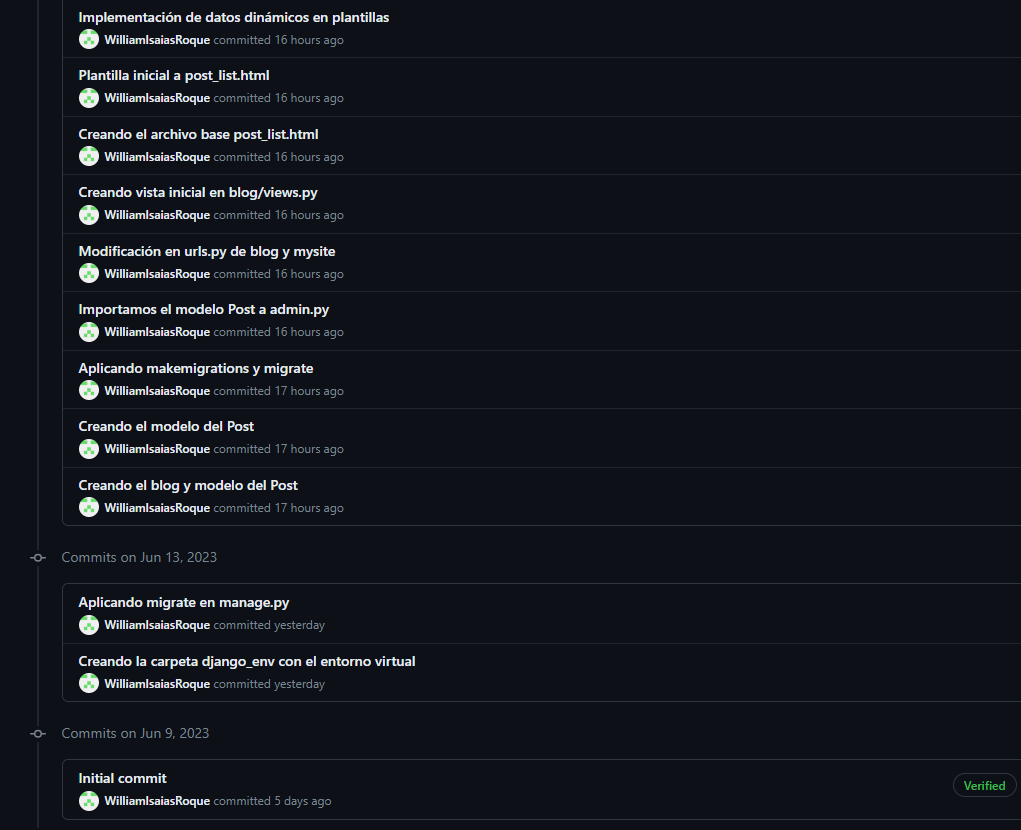
\includegraphics[width=0.7\textwidth]{img/commits1.png}
        \caption*{Primera parte de los commits realizados}
        \end{figure}
        \begin{figure}[ht]
        \centering
        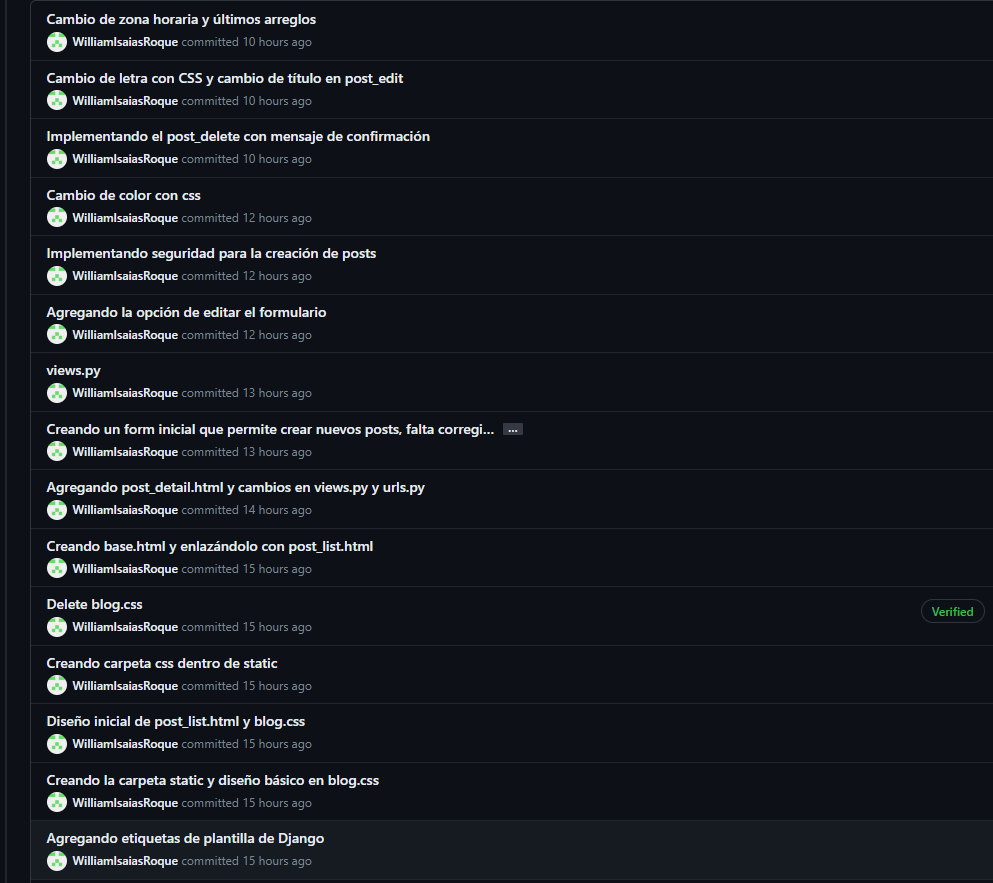
\includegraphics[width=0.7\textwidth]{img/commits2.png}
        \caption*{Segunda parte de los commits realizados}
        \end{figure}
        
        \clearpage
 \section{Cuestionario}
	\begin{itemize}
		\item ¿Cuál es un estándar de codificación para Python? Ejemplo: Para PHP en el proyecto Pear? \\ \\
		PEP 8 es el estándar de codificación que es más aceptado para Python. Proporciona directrices para escribir código legible y consistente, como el uso de indentación de cuatro espacios, líneas de código limitadas a 79 caracteres, nombres de variables en minúsculas separados por guiones bajos, comentarios claros y concisos, importaciones ordenadas, espacios en blanco consistentes y convenciones de nombres.
		\item ¿Qué diferencias existen entre EasyInstall, pip, y PyPM? \\ \\
		EasyInstall fue una herramienta anteriormente utilizada en Python para instalar paquetes y gestionar dependencias. Fue desarrollada por el proyecto setuptools y permitía descargar e instalar fácilmente paquetes desde PyPI. Sin embargo, EasyInstall ha sido reemplazado por pip, que se ha convertido en la herramienta estándar para la gestión de paquetes en Python debido a su mayor funcionalidad y soporte continuo. PyPM, por otro lado, es una herramienta específica de ActivePython que proporciona su propio sistema de gestión de paquetes para la distribución de paquetes de Python en ese entorno particular.
		\item En un proyecto Django que se debe ignorar para usar git. ¿Qué otros tipos de archivos se deberían agregar a este archivo? \\ \\
		Archivos de configuración local: Si hay archivos de configuración local que contienen información sensible como claves secretas, contraseñas u otros datos específicos del entorno de desarrollo, es importante agregarlos al .gitignore para evitar su exposición accidental. Ejemplos comunes son settings\_local.py o secrets.json.
            \item Utilice python manage.py shell para agregar objetos. ¿Qué archivos se modificaron al agregar más objetos? \\ \\
            Al utilizar python manage.py shell en un proyecto Django para agregar objetos a través de la consola interactiva, los archivos que suelen modificarse son los archivos de código fuente de las aplicaciones, como models.py, views.py y forms.py, donde se agregan las definiciones de los nuevos objetos. Además, también pueden generarse archivos de migración en el directorio migrations, reflejando los cambios en la estructura de la base de datos. Estas modificaciones aseguran que los nuevos objetos y su lógica asociada se integren correctamente en el proyecto Django.
            Generalmente se modifican dos tipos de archivos:
            \begin{itemize}
                \item - Archivos de código fuente: Tal es el caso de models.py, views.py o forms.py.
                \item- Archivos de migraciones: Tienen el nombre de 00x\_nombre\_migracion.py, cada archivo de migración tiene un número secuencial. 
            \end{itemize}
	\end{itemize}	
 \section{Referencias}
	\begin{itemize}			
		\item \url{https://tutorial.djangogirls.org/es/django_start_project/}
		\item \url{https://docs.python.org/}
		\item \url{https://realpython.com/python-django-blog/}
	\end{itemize}	
			
\end{document}